\scanpage{6}
% L1
\uline{Démonstration}\qquad 1) On sait, par les généralités sur les
% L2
polyèdres réguliers, que les conditions a) b) impliquent
% L3
l'existence d'un $2$-polyèdre régulier \inserted{paramétré} épinglé, donnant lieu à
% L4
la repr. $\widehat\varphi:G_2\ (\text{groupe cartographique})\longrightarrow\deleted{\unsure{G}}\Gamma\xrightarrow{\varphi}G(S)$, \deleted{d'où on}
% L5
\deleted{déduit, on l'a vu, que $\alpha_0+2,\alpha_1+2,\alpha_0+\alpha_1$ sont inversibles.}
% L6
défini à isom unique près. Un calcul immédiat
% L7
donne que les invariants $\alpha_0,\alpha_1$ de ce $2$-polyèdre ne sont
% L8
autres que $\alpha_0(\varphi)$ et $\alpha_1(\varphi)$. En effet, dans le contexte général
% L9
(dim $n$) avec paramètres $\beta_i=\alpha_i\unsure{+2|-2}$, on a pour $0\leq i\leq n-1$
% L10
\[ f(a_i)=(\beta_0\cdots\beta_{i-1})\quad f(a_{i+1})=\beta_0\cdots\beta_i\quad \varphi(a_i,a_{i+1})=-(\beta_0\cdots\beta_{\unsure{i|i-1}}) \]
% L11
donc si les $\beta_i$ \deleted{sont inv.} \inserted{ainsi que 2,} on peut \deleted{\unsure{faire}} parler de ``l'angle'' $\theta_i$
% L12
de $a_i$ et $a_{i+1}$, on aura
% L13
\[4\cos^2\theta_i=\frac{\varphi(a_i,a_{i+1})^2}{f(a_i)f(a_{i+1})}=\beta_i\qquad(\underline{\mathrm{NB}}\ \zeta_i=\frac{\beta_i}{\mu_i\mu_{i+1}}=\frac{\beta_i}{4}=\cos^2\theta_i).\]
% L14
\[\text{i.e.}\qquad\alpha_i=2(\underbrace{2\cos^2\theta_i-1}_{\cos2\theta_i})=2\cos2\theta_i\]

% L15
Il faut \unsure{donc prouver|au préalable|aussi prouver} ceci :

% L16
\uline{Lemme} (\deleted{\unsure{si car $\ne2$}}\inserted{si $2$ inv}) Soit $(V,f)$ un module quadratique
% L17
lisse de rang $3$, considérons une rotation \deleted{\unsure{de l'axe}} $\rho$
% L18
d'angle $\deleted{\unsure{\theta_i,\,2\theta_i}}\vartheta$ (autour d'un axe tot\textsuperscript{t} non isotrope)
% L19
et soit $\alpha=2\cos\vartheta$. \deleted{Alors} Soit \deleted{\unsure{$Q$}} $Y\subset\check{\mathbb P}(V)$ fibré
% L20
\deleted{des} droites projectives défini par $f$, et considérons
% L21
l'autom $\rho_Y$ \unsure{induit $\rho$|induit} par $\rho$. Ceci posé, l'invariant
% L22
de $\rho_Y$ est donné par
\figure{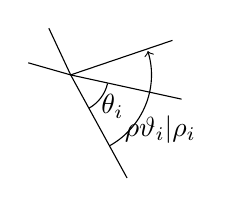
\begin{tikzpicture}[scale=.77]
\draw (-.7,.2)--(0,0)--(1.83,-.40);
\draw (-.36,.77)--(0,0)--(.93,-1.70);
\draw (0,0)--(1.68,.57);
\draw (.30,-.55) arc[start angle=-61,end angle=-13,radius=.63];
\node at (.69,-.52){$\theta_i$};
\draw[->] (.64,-1.17) arc[start angle=-61,end angle=17,radius=1.34];
\node at (1.48,-.90){$\deleted{\unsure{\rho}}\unsure{\vartheta_i|\rho_i}$};
\end{tikzpicture}}
% L23
\[ A(\rho_Y)=\alpha \]

% L24
\uline{Dém} Quitte à choisir des axes de coordonnées convenables
% L25
(possible loc fppf) \deleted{\unsure{SPS}} $f(x,y,z)=x^2+yz$,
% L26
$\rho_{\zeta}(x,y,z)=(x,\deleted{\unsure{\zeta_i}}\zeta y,\zeta^{-1}z)$, et $\alpha=\zeta+\zeta^{-1}$. Or l'hom
% L27
$G_m\hookrightarrow G=\mathrm{Aut}\ C$, $\zeta\unsure{\mathbin{-}|\mapsto}\rho_{\zeta}$, est mono, donc on
% L28
trouve $A(\rho_\zeta)=\zeta+\zeta^{-1}=\alpha$, cqfd.
% archive sheet number: 5
